\documentclass[a4paper, 11pt]{article}
\usepackage{lipsum} %This package just generates Lorem Ipsum filler text. 
\usepackage{fullpage} % changes the margin
\usepackage{mathpazo}
\usepackage[english]{babel}
\usepackage{fontspec}
\usepackage{multicol}
\usepackage{graphicx}
\usepackage{enumerate}
\usepackage{amsmath,amsfonts,amsthm} % Math packages
\usepackage{booktabs}
\usepackage{indentfirst}

\begin{document}
\noindent
\large\textbf{Homework 1} \hfill \textbf{Zhanghao Wu (516030910593)} \\
\normalsize {\bf CS391 Computer Networking} \hfill ACM Class, Zhiyuan College, SJTU\\
Prof.~{\bf Yanmin Zhu} \hfill Due Date: Oct 9, 2018\\
TA.~{\bf Haobing Liu} \hfill Submit Date: \today

\section*{P1}
\subsection*{Massages}
Considering the actions the ATM should take, I design the messages in Table \ref{tab:atm} for the protocol.
\begin{table}[htbp]
	\centering
	\caption{Massages from ATM to centralized computer}
	\label{tab:atm}
	\begin{tabular}{@{}ll@{}}
		\toprule
		Message (\textit{data})   & Description                                                                   \\ \midrule
		LOGIN (\textit{card\_id}) & Inform centralized computer that a card with \textit{card\_id} is in the ATM \\
		PWD (\textit{password})   & User enters the password and ATM sends it to centralized computer            \\
		BALANCE                   & User queries balance                                                        \\
		WDW (\textit{amout})      & User requests withdrawing \textit{amount} of money                           \\
		BYE                       & User is done                                                                 \\ \bottomrule
	\end{tabular}
\end{table}

In response, the centralized computer of the bank may need the messages in Table \ref{tab:cc}.
\begin{table}[htbp]
	\centering
	\caption{Massages from centralized computer to ATM}
	\label{tab:cc}
	\begin{tabular}{@{}ll@{}}
		\toprule
		Message (\textit{data}) & Description                                                     \\ \midrule
		PWD                     & Ask for password of the card                                 \\
		OK                      & Tell the ATM that the last action ends in good for PWD or WDW  \\
		ERR                     & Tell the ATM that the last action ends in error for PWD or WDW \\
		AMT (\textit{amount})   & Response to BALANCE                                          \\
		BYE                     & Permit the ATM to give back the card and return to home page \\ \bottomrule
	\end{tabular}
\end{table}

\subsection*{Assumptions}
Assumptions made by my protocol are shown below:
\begin{enumerate}
    \item The connection between the ATM and the centralized computer of the bank will never disconnected.
    \item The communication between the ATM and the centralized computer of the bank is safe that no fake massage will be accepted and none of the massages can be duplicated.
    \item The application on each side will never get the same massage twice.
\end{enumerate}
\newpage
\subsection*{Diagram}
The case of a simple withdrawal with no errors is shown in the Figure \ref{fig:com}
\begin{figure}[htbp]
    \centering
    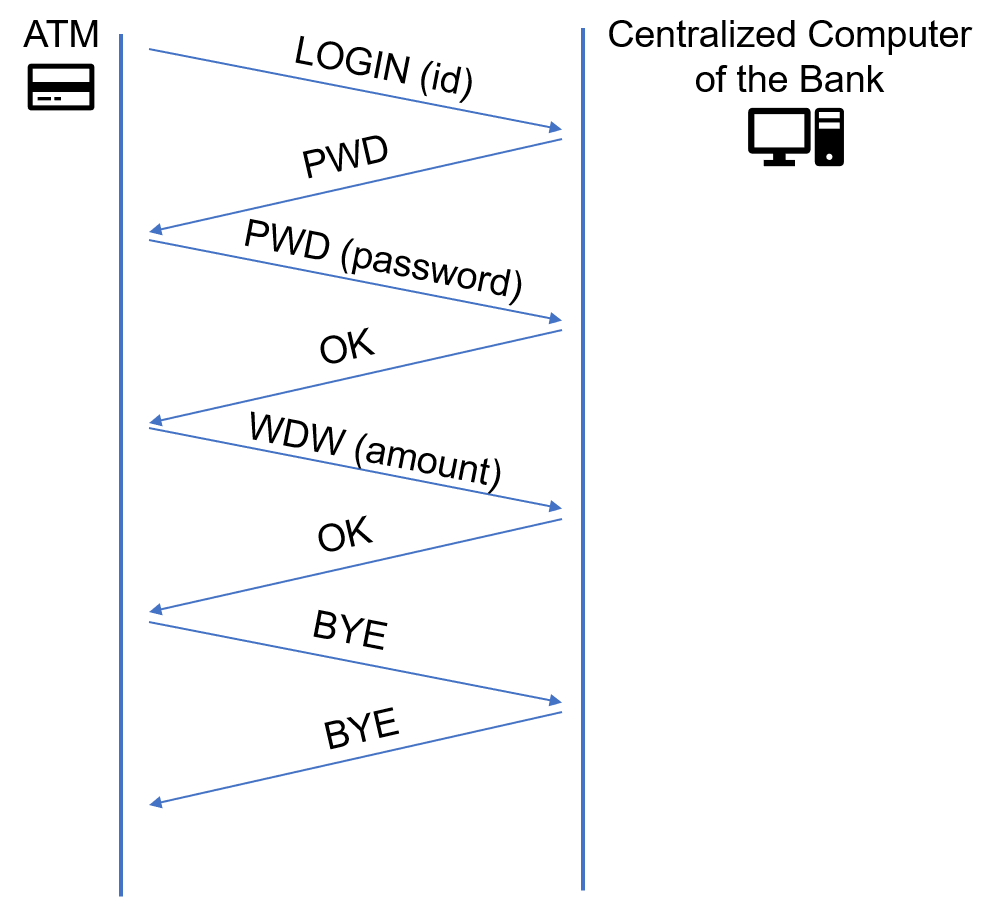
\includegraphics[width=.6\linewidth]{./communication.png}
    \caption{A simple withdrawal with no errors}
    \label{fig:com}
\end{figure}


\section*{P2}
For sending P packets back-to-back over the N links, firstly, we consider the total time the $P^{th}$ packet should wait to be sent. Evidently, for the $i^{th}$ packet, it should wait $L/R$ since the $i-1^{th}$ packet starts transmission. Therefore, the $P^{th}$ packet should wait $(P-1)L/R$ to start transmission. And the time the $P^{th}$ packet take to travel thru the N links is $NL/R$. Therefore, the total time for sendding $P$ such packets back-to-back over the N links is $(N+P-1)L/R$. 

\section*{P9}

\begin{enumerate}[a.]
    \item The maximum number of users that can be supported simultaneously under circuit switching is $N = 1Mbps/100kbps = 10$
    \item The probability for exactly i users are sending data is $\binom{i}{M}p^i$. Therefore, the probability that more than N users are sending data equals to $\sum_{i=N}^{M}\binom{i}{M}p^i$
\end{enumerate}
\newpage
\section*{P14}
\begin{enumerate}[a.]
    \item As each packet consists of L bits, the transmission delay is $\frac{L}{R}$. Therefore, the $\text{total delay} = \text{queuing delay} + \text{transmission delay} = \frac{IL}{R(1-I)} + \frac{L}{R} = \frac{L}{R(1-I)}$
    \item Let $x = \frac{L}{R}$. Then the total delay is $\frac{x}{1-ax}$. And the plot of the function are shown in Figure \ref{fig:del}.
        \begin{figure}[htbp]
            \centering
            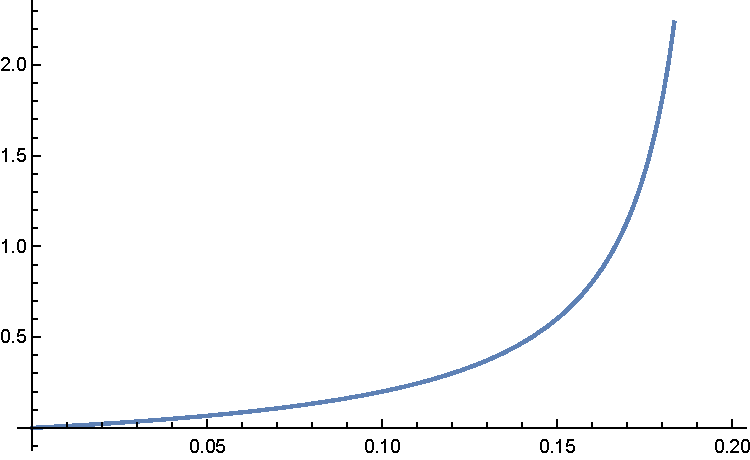
\includegraphics[width=.6\linewidth]{plot.pdf}
            \caption{The total delay function (a=5) with respect to $\frac{L}{R}$}
            \label{fig:del}
        \end{figure}
\end{enumerate}

\section*{P16}
According to the problem, the $\text{transmission delay} = \frac{1 \text{ packet}}{\text{transmission rate}} = 10\text{ msec}$. Therefore, $d=\text{transimission delay} + \text{queuing delay} = 2\text{ msec}$.Hence, the $\text{average packet arrival rate } a=\frac{N}{d} = \frac{10 \text{ packets}}{0.02 \text{ sec}} = 500 \text{ packets/sec}$

\section*{P25}

\begin{enumerate}[a.]
    \item The propagation delay $\text{dprop} = \text{distance}/\text{propagation speed} = 0.08\text{ sec}$. The bandwidth-delay product$=\text{R}\cdot \text{dprop}=0.16\text{ Mb}$
    \item As $0.16$ M is smaller tha the file size $0.8M$.The maximum number of bits that will be in the link at any given time equals to the bandwidth-delay product, i.e. $0.16$ M
    \item The bandwidth-delay product is the maximum number of bits that can be in the link at a given time.
    \item As there are $0.16$ M bits in the link, the width of a bit in the link is $\frac{2\times 10^7 \text{ meters}}{0.16\times 10^6 \text{ bits}} = 125 \text{ meters/bits}$, which is longer than a football field($120$ meters).
    \item The propagation delay equals $\frac{m}{s}$. And the bandwidth-delay product equals $\frac{mR}{s}$. Therefore the length of a bit is $\frac{m}{\frac{mR}{s}} = \frac{s}{R}$
\end{enumerate}


\end{document}
